\documentclass[
12pt         % Moar bigger
,twoside     % fogs hates this, but they hate everything
,openright   % fogs hates this too
]{mythesis}

% I used these in my thesis.  They're useful.  booktabs makes non-shit
% tables.
\usepackage{graphicx}
\usepackage{amsmath}
\usepackage{booktabs}

\title{Abiotic and biotic factors\\%
  creating variation among\\bromeliad communities}
%
\author{Arthur Andrew Meahan MacDonald}
%
\month{\textsc{august}} \year{2016}
\previousdegrees{B.Sc., Cape Breton University, 2006\\%
  M.Sc., University of Toronto, 2009}
\degreetitle{Doctor of Philosophy}
\department{Zoology}

\begin{document}

\maketitle

% I worked in different files: input them like so:

\chapter*{Abstract}
\chaptermark{abstract}
\addcontentsline{toc}{chapter}{Abstract}

Many ecological communities show variation from place to place; understanding the causes of this variation is the goal of community ecology. Differences in community composition will be the result of both stochastic and deterministic processes. However, it is difficult to know to what degree, and under which circumstances, deterministic processes will shape community composition. In this thesis I combined observational and experimental approaches to quantify deterministic processes within a particular ecological community -- they phytotelmata of bromeliad plants. In my thesis I describe three studies at different scales of organization: 1) do organisms of different size respond equally to changes in their environment 2) how do predators interact to influence prey survival 3) what mechanisms underly the response of similar species to the same environmental gradient, bromeliad size. 

In Chapter 1, I tested an hypothesis developed from previous observational data - that smaller organisms respond less than larger ones to the same environmental gradient -- different bromeliad species that occur under different forest canopies. I placed identical communities of bacteria, zooplankton and insect communities into bromeliads in different habitats. I found that community composition diverged little for bacteria, more for zooplankton and most of all for macroinvertebrates. In my second chapter, I examined ecological determinism on a smaller scale -- within a single trophic level (macroinvertebrate predators). I found that predators may interfere with each other, reducing predation rates and increasing prey survival. In Chapter 3, I examine macroinvertebrate responses to bromeliad volume. I use a null model to demonstrate that species vary in their response to area more than can be explained by sampling effects alone. Then I discuss a detailed field experiment which showed that for at least one such pair, a difference in abiotic tolerances may be the plausible mechanism. 

Together these results illustrate when, and to what degree, bromeliad communities respond to deterministic factors. All three chapters first demonstrate a pattern, testing it against a suitable null distribution, before attempting to quantify possible mechanisms with a field experiment. This combination of observation and experiment is an approach which can contribute to our understanding of how ecological systems work. 
%%% Local Variables:
%%% TeX-master: "thesis"
%%% TeX-PDF-mode: t
%%% End:

\chapter*{Preface}
\addcontentsline{toc}{chapter}{Preface}

All three chapters in this thesis are original work. The ideas for all chapters were developed by A. A. M. MacDonald and supervisor D. S. Srivastava and were written by A.A.M.M.D. as manuscripts and edited by the co-authors.  Chapter 2 is co-authored with D. S. S., Vinicius Farjalla and Flavia Lima and Alice Campos. V.F. contributed field support and advice on experimental design, while F.L. performed the DGGE analysis of bacterial diversity and A.C counted protists. Chapter 3 is co-authored with D. S. S. and G. Q. Romero, who contributed to the ideas and field support. Chapter 4 is co-authored with D. S. S., who also collected the observational data used in that chapter, while A.A.M.M.D. collected the experimental data.  Field work was completed by A.A.M.M.D. with field assistants Aline Nishi (Chapter 3) and Pedro Trasmonte (Chapter 2 and 4).  All programming and analysis for all chapters was completed by A.A.M.M.D.

%%% Local Variables:
%%% mode: latex
%%% TeX-master: "thesis"
%%% TeX-PDF-mode: t
%%% End:

% This is because FoGS formatting pedandtry is especially accute when
% it comes to tables of contents
\allcontents
% There is currently a problem with spacing somewhere so that Table of
% Contents, List of Tables, and List of Figures have the wrong amount
% of space.  Others are OK though...
\chapter*{Acknowledgements}
\addcontentsline{toc}{chapter}{Acknowledgements}

Acknowledgements are the hardest part of a thesis to write because
they're the only bit most people read.

%%% Local Variables:
%%% TeX-master: "thesis.tex"
%%% TeX-PDF-mode: t
%%% End:

\cleardoublepage
\phantomsection
\addcontentsline{toc}{chapter}{Dedication}
\vspace*{.1\textheight}
\begin{center}
  To Angela
\end{center}

\cleardoublepage
\mainbody

\chapter{Introduction}
\label{chap:introduction}

% Yay inspiriational quotes.
% \begin{quoteshrink}
%   ``At yet higher levels, the species and the community, natural
%   selection obviously must occur. Species evolve to survive in a certain
%   environmental range, and if the environment should suddenly change,
%   some species will become extinct but others will survive.''
%   \hfill\citet{Lewontin-1970-1}, p.~15
% \end{quoteshrink}

\noindent

Observation and experiment are the two fundamental approaches to
understanding ecological systems. In this thesis I use a combination of
observation, null models, and experimental manipulation to understand
what structures aquatic communities in bromeliads. Observational data
are a critical first step in documenting patterns in the natural world.
Null models enhance observational data, as they attempt to represent how
these patterns may have occurred in the absence of a particular
ecological process. As such, when observations exceed the bounds of a
null model, they offer a tantalizing suggestion that the proposed
process might actually be occurring. Experiments can then identify and
isolate which precise process is occurring, and measure its magnitude.
Process is essential to our ability to generalize our results beyond any
one specific system.

But which processes generate patterns of biodiversity in nature that
ecologists seek to explain? Vellend \citep{Vellend2010b} contends that
the myriad of different processes that determine ecological communities
can be grouped into four categories, analogous to the four processes
which underlie evolutionary change: drift, selection, speciation and
dispersal. These processes interact to create the variation we
see among natural communities. Ecological drift is the temporal
variation in the relative abundances of species caused by the sequence
of demographic events within each species. Dispersal is the movement of
organisms or propagules from the regional pool into a local site, which
can introduce new species into a local community. Speciation introduces
new species simultaneously into a community and the regional species
pool, and ecological `selection' determines which particular species
persist in a local patch. Ecological selection refers to the processes
which result in a higher fitness of a given species in a particular
environment relative to all other species present. The similarity
between this process and that of natural selection within a population
is only an analogy, substituting the performance of species for those of
genes. The deterministic nature of ecological selection results in a
nonrandom association between either species and the environment, or
species and each other.

Ecological selection can be predicted by morphological and behavioural
traits of organisms -- i.e., their functional traits. This assumes the
existence of niche-based processes in structuring communities. The niche
is the combination of resource concentrations, and abiotic and biotic
conditions that allow a population to persist. Since the phenotype of
organisms determines the response of the organism to particular
resources or conditions, it stands to reason that the different traits
of organisms then relate to their niche. Traits, however, are
notoriously difficult to measure. Ecologists have therefore proposed
phylogeny as a possible substitute for detailed trait information. This
approach assumes that similarity between species in
ecologically-relevant traits is correlated with the amount of shared
evolutionary history. Phylogeny may go beyond being a (questionable)
substitute for measured traits, and even represent traits which are
difficult to measure \citep{Cadotte2008, Srivastava2012c}. Thus,
nonrandom patterns of either phylogeny or traits are often used as a
means of identifying where niche-based processes are operating. However,
this is not always the case \citep{Mayfield2010}.

The four general categories of ecological processes probably operate in
every system on Earth. However, they cannot be studied everywhere,
usually because of the ``problem of scale'' \citep{Levin1992}: many
systems are too big, or too slow to develop. Therefore, several
empirical ecologists have pursued the study of smaller, simpler systems
(often referred to as ``mesocosms'' or ``microcosms'', to separate them
from larger and more complex systems. This has often been argued to be
the case for natural \citep{Srivastava2004a} and artificial
\citep{W.Fox2007} mesocosms and microcosms. Bromeliads are a key system
because their small size makes them tractable to rapid observation and
manipulative experiment. Bromeliads are home to a wide variety of
animals. These animals interact in a complex food web including
competitors, predators, and even mutualists. Although the habitats are
small, they are neither homogeneous nor very similar to each other --
bromeliads are found in a staggering variety of sites and microhabitats.
Even within a habitat, they span several orders of magnitude in size,
from very small (\textasciitilde{}10ml) to very large (\textgreater{}5L)
plants.

\begin{figure}[htbp]
\centering
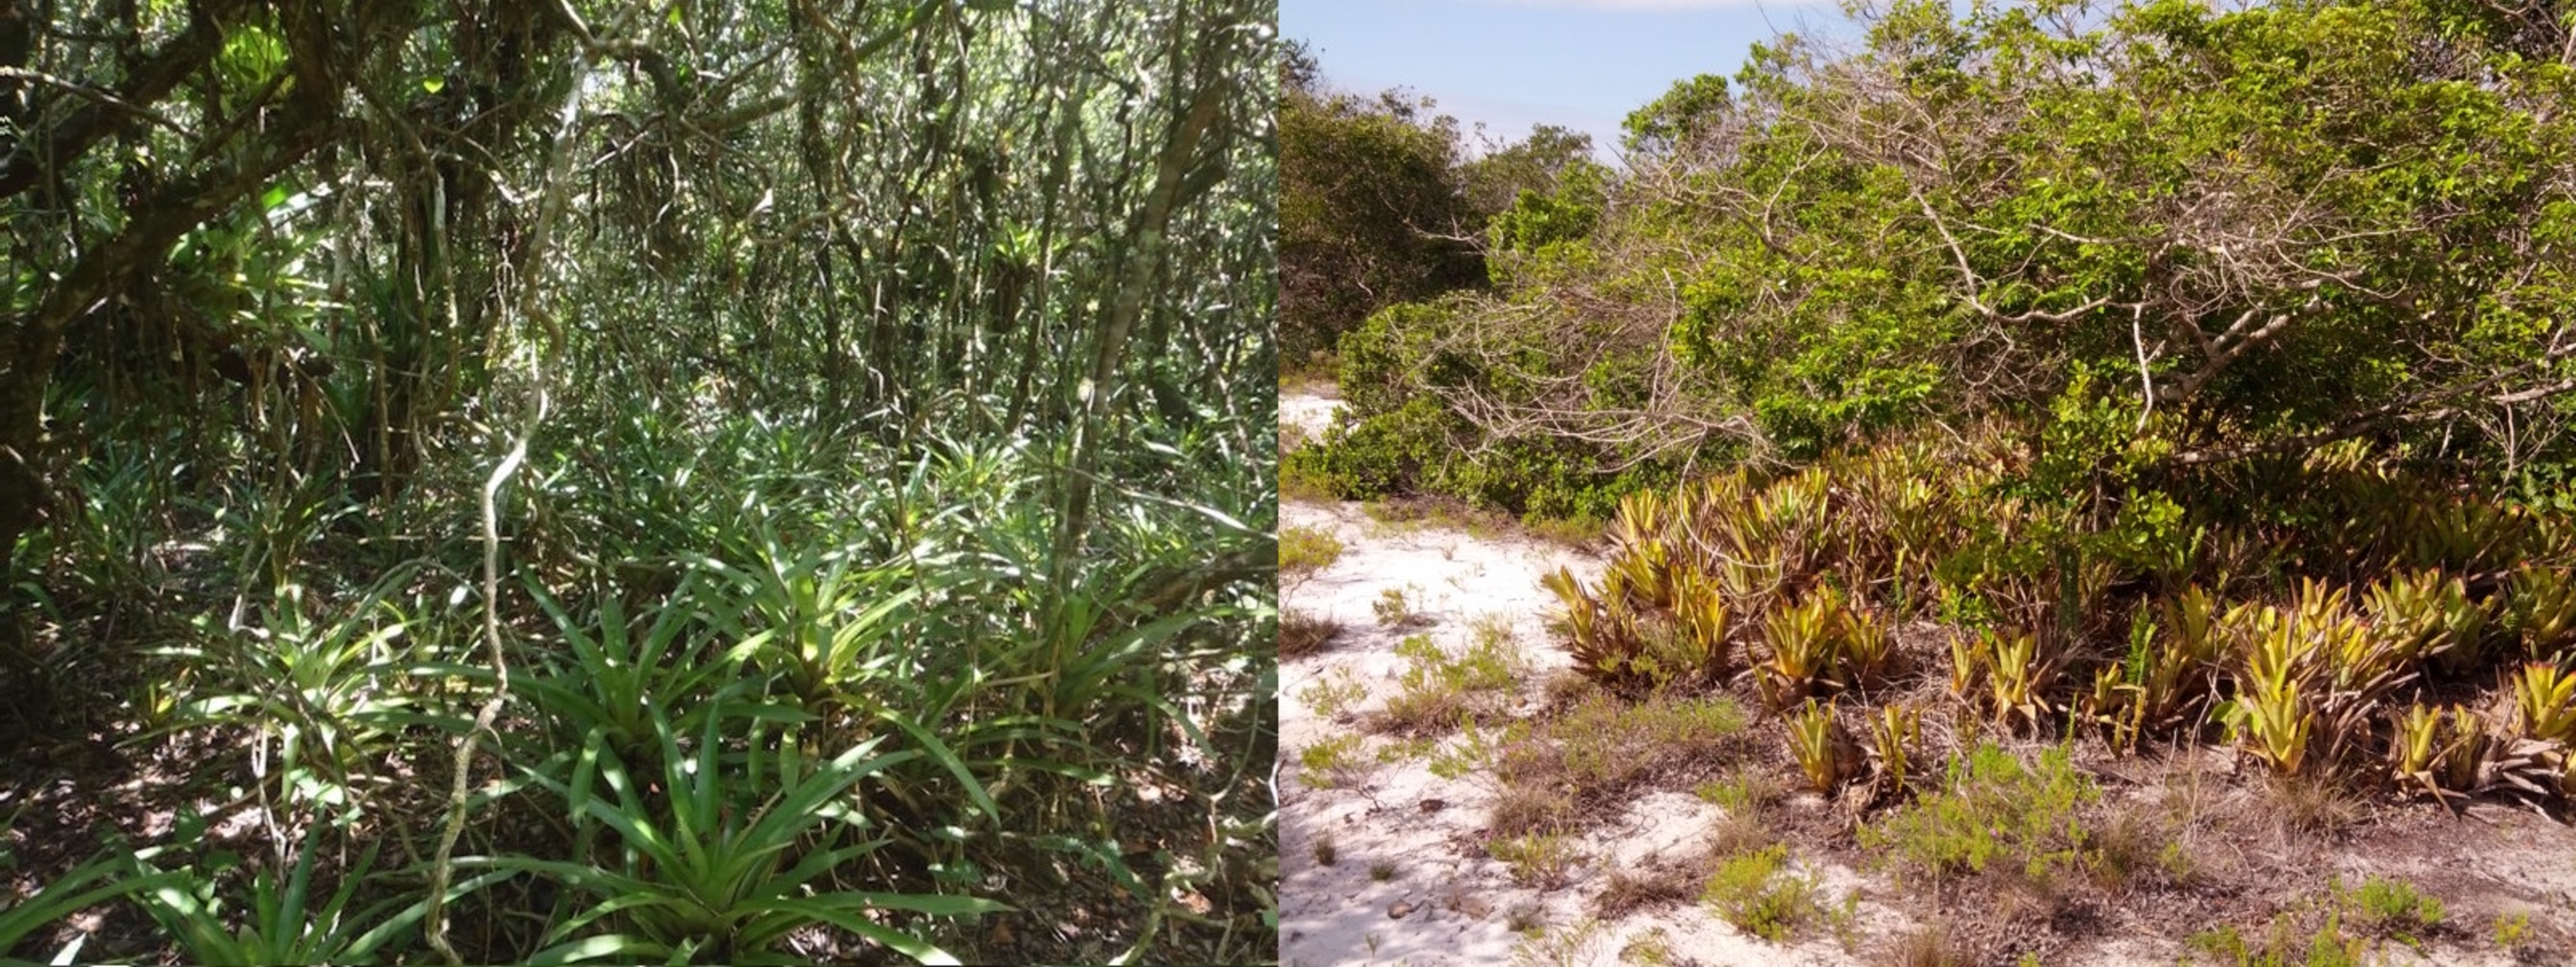
\includegraphics[width=5.5in]{figures/restinga2.pdf}
\caption[Photos of \emph{restinga} vegetation in Brazil]{Photos of \emph{restinga} vegetation in Brazil. \emph{Restingas} are dry, sandy habitats that occur in coastal sites within the Atlantic Rainforest in Brazil. On the left is a forested or ``closed'' restinga which was the location for Chapters 3 and 4. On the right is a more exposed or ``open'' restinga, the site of Chapter 2}
\label{fig:phylo_niche_overlap}
\end{figure}


In this thesis, I take the approach outlined above and apply it to the
tractable model system of bromeliad food webs. I use a combination of
observations and experiments to examine how deterministic and stochastic
processes affect the structure and functioning of these communities. In
each chapter I compare observations against specific null models, to
estimate which processes might be at work. Then, using manipulative
experiments, I test mechanisms suggested by the null models. I examine
two sources of ecological selection: the environment (abiotic) or other
organisms (biotic). Differences in the abiotic environment select for
the presence of different species; this is called habitat filtering.
Habitat filtering has many meanings \citep{Southwood1977, Kraft2015} but
in general refers to a conceptually simple process: among those subset
of species which arrive in a given patch, those who persist must be able
to tolerate both the abiotic and biotic conditions of that patch.

In Chapter 2, I consider the question of which types of organism
(bacteria, zooplankton or macroinvertebrates) show the strongest degree
of habitat filtering. Here, bromeliads offer a rare opportunity to
compare the community structure of these three organisms types -
differing in body size by many orders of magnitude- over the exact same
habitat gradient. In Chapter 3, I first identify the frequent
co-occurrence of predators with one another in bromeliads and overlap in
diets. This suggests the potential for strong predator-predator
interactions, which theoretically can have both antagonistic and
synergistic effects on prey. I use this as an opportunity to determine
how the phylogenetic diversity of predators affects their impact on prey
and ecosystem functions. In Chapter 4, I analyze the differences between
two congeneric species which have very different responses to habitat
size. In this chapter, I also demonstrate that invertebrate species that
live in bromeliads have a strikingly different response to bromeliad
size.

%%% Local Variables:
%%% TeX-master: "thesis"
%%% TeX-PDF-mode: t
%%% End:

\chapter{Smaller organisms are less strongly structured by environmental variation}
\label{chap:organism-size}

\subsection{Introduction}\label{introduction}

One of the most profound differences between organisms is their body
size. Small and large organisms can differ in population size, growth
rates, morphological complexity, genome size, and modes of dispersal.
This scaling of biological processes with organism size has often been
used to explain differences in the spatial distribution of small and
large organisms. Microscopic organisms such as bacteria and plankton are
often globally distributed, while larger organisms have more
geographically restricted distributions \citep{Fenchel2004}. Even within
landscapes, there is some evidence that the occurrence of such
microscopic organisms responds less to environmental gradients than does
the occurrence of larger organisms \citep{Farjalla2012, Fierer2011}.
However, while such differences in distribution suggest that the suite
of processes underlying community assembly differ between small and
large organisms, it is difficult to determine which process is driving
this difference. There are at least two possible mechanisms that may
make communities of smaller organisms more widely distributed. First,
smaller organisms could have larger environmental tolerances, allowing
them to occupy broader fundamental niches. Second, smaller organisms
could have greater dispersal abilities, allowing them to reach more
habitats.

Smaller organisms may have broader environmental tolerances for several
reasons. First, their small body size allows habitat heterogeneity to
affect them at very small scales: smaller organisms are able to find
tolerable microhabitats, while organisms that experience the environment
at a coarser grain may not detect a similar variation in the
environment. This biological difference between small and large
organisms can be compounded by the macroscopic grain at which organisms
are typically observed by researchers, which averages over any
microscopic-scale variation in distribution. Secondly, single-celled
organisms may be able to use multiple carbon sources
\citep{Langenheder2007} allowing them to survive in a greater range of
habitats. Very small organisms are also more likely to possess resting
stages when a habitat is unfavorable (e.g.~cysts for protists, tun state
for tardigrades) or to propagate by means of a resistant life history
stage such as spores. At the population level, small organisms may
persist in a habitat if they are able to adapt to local conditions by
virtue of their short generation times and high population sizes. In the
case of bacteria, genetic adaptation can also involve the uptake and use
of environmental DNA.

Alternatively, small organisms may be widely distributed because they
are able to get to more places faster. There is substantial evidence
that microscopic organisms such as bacteria, viruses, protists and
plankton may be able to disperse further than larger organisms; amongst
these microscopic organisms, the smallest disperse the furthest. The
classic ``everything is everywhere and the environment selects''
hypothesis of Baas Becking \citeyearpar{BaasBecking1934} suggests that
smaller organisms are not limited by dispersal barriers or distance but
instead are found globally, emerging from resistant stages in favorable
environments \citep{Huszar2015}. Many bacteria and zooplankton have
passive dispersal, traveling long distances by wind or water currents,
or by phoresy. In contrast, larger animals (but not larger plants)
usually have active dispersal; for example, adult insects actively
choose sites to oviposit. At the scale of landscapes, active dispersal
could result in a close association between distribution and
environmental variables, assuming that active dispersal behaviour is
adapted to maximize fitness. However, at continental and global scales,
the limited distances covered by active dispersers might prevent larger
animals from reaching suitable places. This would weaken the association
between environment and distribution for larger animals.

It has been difficult to determine whether differences in distribution
between small and large organisms is caused by differences in the
strength of environmental filtering or dispersal limitation. There are
three reasons for this. First, the distribution of micro-and macroscopic
organisms has rarely been compared within the same system. This creates
a problem of scale, with studies of many macroscopic organisms occurring
on much smaller spatial scales than those of microscopic organisms.
Second, when we rely on observational data alone, we have a limited
ability to infer environmental filtering. This is because environment,
space and dispersal are often correlated. Previous researchers have used
variance partitioning to separate the effects of environment from space,
but this approach has limitations \citep{Gilbert2010}. For example,
Smith and Lundholm \citeyearpar{Smith2010} found that
spatially-correlated dispersal contributed to both spatial and
environmental partitions of variance in community composition. Third,
dispersal limitation and environmental filtering can mask each other. A
species can only be filtered by a site's environment when it can reach
the site, so a community experiencing equally strong dispersal and
environmental limitation can may show mainly the former in variance
partitioning \citep{Smith2010, DeBie2012a}. A special case of this
problem occurs when an actively-dispersing species is not found in a
site. It is impossible to determine if this is because the environment
makes dispersal unlikely or establishment unlikely. For example, an
insect larva may be missing from a location because its parent was
deterred from ovipositing in the environment or because the larvae could
not withstand the environment. An experiment that removes dispersal
limitation for all organisms is therefore a stronger test of the
relative effects of environment on species composition. We are aware of
no study that experimentally removes dispersal limitation for both
micro- and macroscopic organisms in the same system, simultaneously, to
reveal environmental filtering. We conducted such an experiment, using
bromeliad phytotelmata as a model community.

Here we provide a robust test of the strength of environmental filtering
for these three organism types by experimentally dispersing all species
to all habitats, and examining whether the original habitat-based
patterns in composition re-emerged. We predicted:

\begin{enumerate}
\def\labelenumi{\arabic{enumi}.}
% \tightlist
\item
  If environmental filtering, but not dispersal limitation, increases
  with organism size, we would predict that habitat would affect the
  composition of communities of large-bodied organisms more than those
  of small-bodied organisms(Figure 1a). 
\item
  If instead only dispersal limitation increased with organism size, we
  would expect that any apparent effect of habitat on community
  composition was an artifact of spatial autocorrelation and would be
  erased by our removal of dispersal limitation (Figure 1b).
\item
  If both environmental filtering and dispersal limitation increased
  with organism size, we would predict an intermediate scenario (Figure
  1c).
\end{enumerate}

\subsubsection{Study system}\label{study-system}

Bromeliads are common in the Neotropics and contain many species of
macroinvertebrates, especially insects \citep{Frank2009}, zooplankton
\citep{Petermann2015}, and bacteria \citep{Haubrich2009a}. Importantly,
different species of bromeliad grow in different habitats, and this
habitat variation is correlated with differences among their communities
\citep{Marino2012}. Previous observations in this system show that this
environmental variation is closely associated with variation in
macroinvertebrate composition, weakly associated with variation in
zooplankton communities and almost uncorrelated with variation in
bacterial communities \citep{Farjalla2012}.

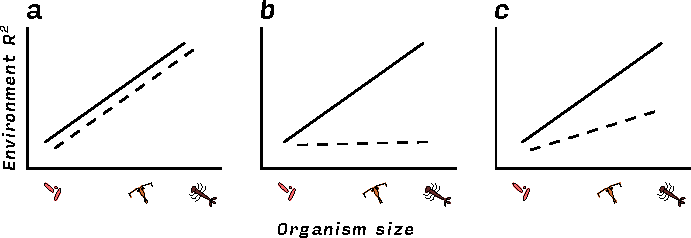
\includegraphics{figures/hypotheses_illustration.pdf}

Figure 1: Illustration of the possible patterns resulting from our
experiment. Previous observations have already shown that community
composition of larger animals is more strongly related to environmental
differences than is composition of smaller organisms (solid line, all
figures). In our experiment we remove differences among community
composition, and observe the subsequent return of these differences as
caused by environment (dashed lines). There are three possible outcomes.
If differences in composition are caused by an increase in sensitivity
to the environment (with increasing organism size), then we should see a
match between the amount of environmental signal before and after the
experiment (1a). If differences in composition are caused by biased
dispersal, we should see no difference between organism types after the
experimental homogenization (1b). Finally, an intermediate scenario (1c)
results when both environment and biased dispersal contributed to the
original pattern.

\subsection{Methods}\label{methods}

\subsubsection{Experimental design}\label{experimental-design}

We performed this experiment in the same location and along the same
gradient of environmental variation (bromeliad species in different
habitats) as Farjalla et al. \citeyearpar{Farjalla2012}. Both their
study and ours took place in the Parque Nacional de Jurubatiba,
Northeast Rio de Janeiro state, Brazil (\(22^{\circ}\) S \(41^{\circ}\)
W). The environmental gradient in this ecosystem is twofold -- three
different species of bromeliad, which differ also in their preferred
level of exposure to sunlight: \emph{Aechmea nudicaulis} (full sun
habitats), \emph{Vriesea neoglutinosa} (partial shade), and
\emph{Neoregelia cruenta} (full shade). \emph{Neoregelia} has a uniquely
large habitat range at this site, occurring in both full shade and full
sun; only shade plants were used in this study.

For each of five temporal blocks, we collected and sampled the
macroinvertebrates, zooplankton and bacteria of two bromeliads of each
of the three species. We then homogenized the communities of all six
bromeliads as described shortly (Figure 2). Our goal was to create
identical starting community composition for all bromeliads within a
block. Variation between blocks in starting community composition is
thus included in the random effect of blocks. We created five blocks in
this experiment between 27 March 2013 and 03 April 2013.

\begin{figure}[htbp]
\centering
\includegraphics{figures/design_illustration.pdf}
\caption{img}
\end{figure}

Figure 2: Schematic of our experimental design. We first sampled six
bromeliads (two plants of each of three species). We formed (solid
arrows) homogeneous initial communities (MIX) by counting equal numbers
of animal taxa (macroinvertebrates) or by mixing water samples of equal
volume from all plants (zooplankton and bacteria). We then returned
(dashed arrows) initial communities to the six bromeliads in their
associated habitats.

Our experimental setup consisted of three steps (Figure 2): collection
of original communities from bromeliads, homogenization of communities,
and assembly of this homogenized community in each of the original (now
empty) bromeliads. \textbf{Original communities}: We sampled the
zooplankton and bacteria communities by collecting water samples from
each bromeliad: 100ml for zooplankton, 50ml for bacteria. Zooplankton
were collected by filtering on 50 μm Nytex mesh and fixed in 5\%
buffered formalin. This fixed solution was then diluted to 20 ml, and a
1 ml subsample taken for analysis. Zooplankton were identified to the
lowest taxonomic unit possible (species in most cases, except for
bdelloid rotifers and harpaticoid copepods, identified to class and
order, respectively). Bacteria were collected by taking 100ml of
filtrate from the zooplankton sample and filtering it a second time on a
Whatman filter paper. We measured bacterial community composition using
denaturing gradient gel electrophoresis (DGGE, Muyzer et al.
\citeyearpar{Muyzer1993}). This technique measures an approximation of
bacterial diversity in the form of Operational Taxonomic Units (OTUs).
We sampled macroinvertebrates by thoroughly rinsing each bromeliad and
filtering the water through 1mm and 180μm mesh. These mesh sizes have
been shown to separate macroinvertebrates from both coarse detritus and
fine particulate organic matter, facilitating their collection
\citep{Romero2010}. We identified macroinvertebrates to morphospecies.
\textbf{Homogenized communities}: We created homogenized communities of
zooplankton and microbes by mixing an equal volume of filtered tank
water from each of the six bromeliads in a block (approximately 100ml
plant\textsuperscript{-1}), then adding this mixture to all bromeliads.
To create homogenized communities of macroinvertebrates, we divided
individuals of all species equally among the six bromeliads in each
block. \textbf{Bromeliad preparation}: We emptied bromeliads by washing
them thoroughly, hanging them upside down to dry for at least 24 hours
and then rinsing each plant with 70\% ethanol. We confirmed that this
technique removed all invertebrates and most detritus by dissecting an
empty bromeliad. Any coarse detritus found in the bromeliads was
similarly cleaned, frozen and thawed (to kill any eggs or resting stages
of macroinvertebrates).Bromeliads were placed in a local habitat similar
to their original location: \emph{Neoregelia} in shade, \emph{Aechmea}
in full sun and \emph{Vriesea} in marginal habitat. We then added the
starting communities of macroinvertebrates, zooplankton and bacteria.

Bromeliads are an open system, characterized by continual colonization
and emergence. Both of these processes are problematic for our question.
If we were to allow colonization it could swamp any changes in our
starting community composition. Conversely, if we allowed the experiment
to continue for too long any macroinvertebrates with complex life cycles
would emerge, leaving us with no community to sample \citep{Lecraw2014}.
We took two steps to make sure that our treatment effects were not
affected by colonization or excessive emergence. To prevent colonization
we surrounded bromeliads with mosquito netting (mesh size approx. 1.5
mm). To prevent emergence we ended our experiment after 12 days, based
on the results of a pilot study that confirmed that this was sufficient
time for communities to change, but not so long that bromeliads became
empty of organisms

\subsubsection{Analyses}\label{analyses}

We distinguished between our three predictions (Figure 1) with a
permutational ANOVA (PERMANOVA), which measures the amount of difference
in community composition between treatment groups and compares this to
the expected distribution under a null hypothesis of no treatment
effects. In each PERMANOVA we used block as an error stratum, meaning
that permutations were performed within blocks. We repeated this
analysis for all three organism types, and at both ``initial'' and
``final'' sampling dates (i.e.~at the beginning and end of the
experiment). We interpreted the R\textsuperscript{2} value of this
PERMANOVA as a metric of the strength of habitat filtering (Figure 1).
Our hypothesis predicted that R\textsuperscript{2} values should
increase from smaller to larger organism types. However, because we
sampled each of these groups with different techniques, and collected
different types of data (e.g.~abundance data for macroinvertebrates,
presence/absence for bacterial OTUs) we may observe different
R\textsuperscript{2} values through statistical, not biological,
processes. Therefore we tested a pattern of increasing
R\textsuperscript{2} against the increase that would be expected under
the null hypothesis of no difference in environmental filtering. We
first quantified the upward trend with the slope of a linear regression
of R\textsuperscript{2} as a function of approximate organism size
(bacteria = 0.04mm, zooplankton = 0.5mm, macroinvertebrates = 5mm). To
generate our null distribution, we generated a random permutation of the
environmental variable (i.e.~bromeliad species). We used the same
permutation series for each organism type. We calculated the
standardized effect size of the observed slope with the equation

\(SES = \frac{Slope_{observed} - mean(Slope_{null})}{SD(Slope_{null})}\)

We calculated the null p-value as the proportion of null simulations
equal or greater to the observed slope. All statistical analyses were
conducted in R 3.2.3 \citep{rcore}.

\subsection{Results}\label{results}

Bromeliad species identity explains more variation in community
composition of macroinvertebrates than any other organism type, less for
zooplankton and less still for bacteria (Figure 3, Table 1). For all
organism types, bromeliad species explained less of the variation in
composition at the end of the experiment than at the beginning. Note
that, although the sampling design (and therefore degrees of freedom)
are identical for all groups, the critical (alpha = 0.05) F-value for
each organism group differs because PERMANOVA p-values are calculated on
a null distribution generated by permuting samples among groups (species
in our case). Bacterial communities have many species and also high
similarity among communities (bromeliads), creating a null distribution
with low mean and small variance (and hence lower thresholds for
significance). This increases the power to detect habitat effects for
bacteria, explaining why this group has marginally significant effects
of habitat despite habitat explaining a tiny amount of total variation
in composition.

So far, we have assessed the absolute effect of habitat filtering on
each organism group separately, but our goal was also to determine if
the strength of habitat filtering increases between the organism groups.
We therefore compared this pattern of increasing environmental effects
with a null model. First, we calculated the slope of the relationship
between the R\textsuperscript{2} value and approximate organism size. We
then generated null distributions by reshuffling bromeliad species
within blocks, using the same permutation across all organism types. We
found that the observed slope was much higher than the null simulations
for both initial (SES = 6.18, p = 0.002) and final (SES = 4.82, p =
0.002) sampling (499 simulations).

\subsubsection{Tables}\label{tables}

\begin{center} 
\begin{table}[h] 
\caption[Sample table]{Bromeliad species effects on the composition of three types of
organisms, as determined by PERMANOVAs both before and 12 days after
homogenization. Both before and after homogenization,
R\textsuperscript{2} values (our proxy for the strength of habitat
filtering) are higher for macroinvertebrates than for zooplankton than
for bacteria. Following homogenization, macroinvertebrate and bacterial
communities both significantly diverged among bromeliad species.} 
\label{table:r2s} 
\vspace{10pt} 
\begin{tabular}[c]{l l l l l} 
\hline 
& & F227 & p & R2 \\
macroinvertebrates & before & 7.03 & 0.001 & 0.34 \\
& after & 6.42 & 0.001 & 0.32 \\
zooplankton & before & 2.59 & 0.008 & 0.16 \\
& after & 1.75 & 0.158 & 0.11 \\
bacteria & before & 0.69 & 0.085 & 0.05 \\
& after & 0.63 & 0.027 & 0.04 \\
\end{tabular} 
\end{table} 
\end{center} 


\subsubsection{Figures}\label{figures}

\begin{figure}[htbp]
\centering
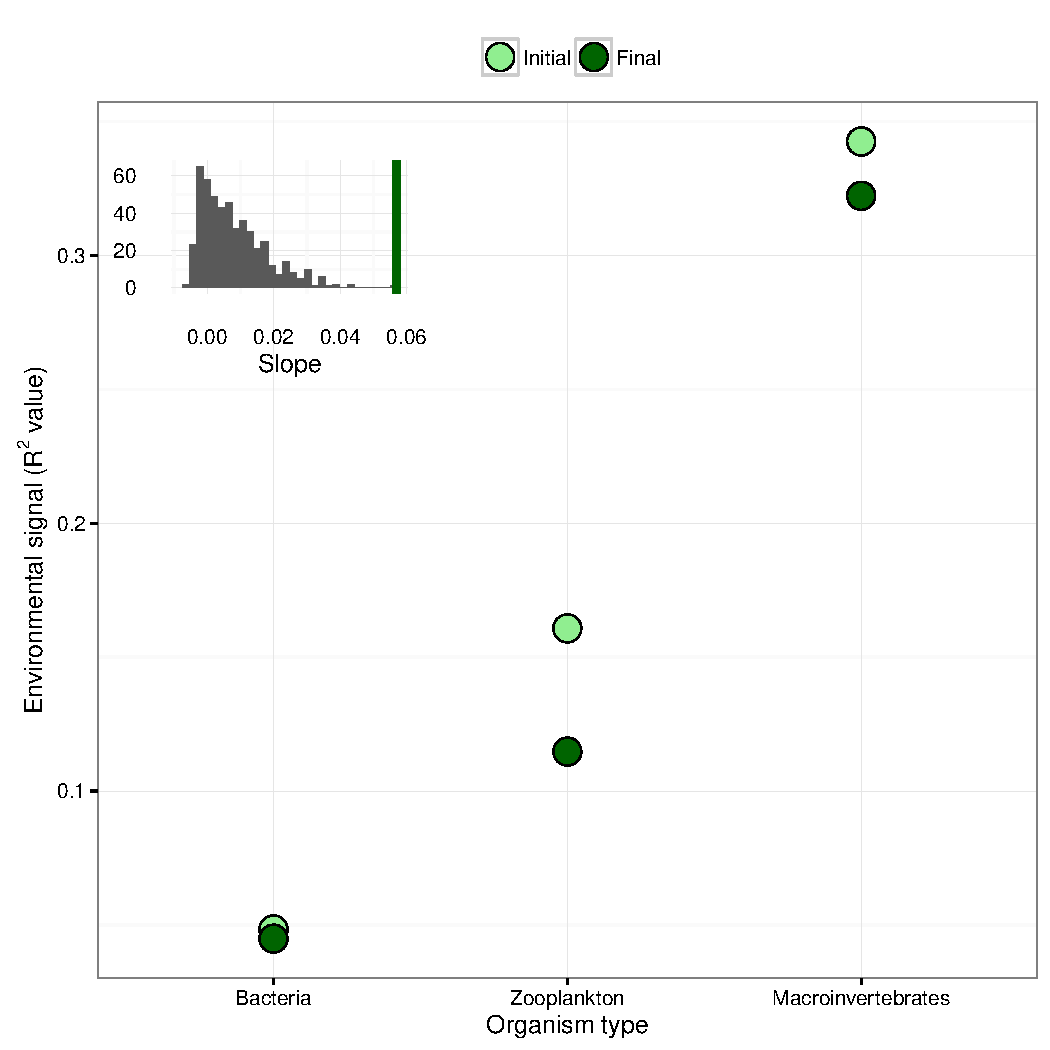
\includegraphics{figures/r2_plot.pdf}
\caption{The amount of variation (R\textsuperscript{2} from PERMANOVA)
in community composition explained by bromeliad species (i.e.~the
strength of the environmental signal) decreases from larger to smaller
organisms. The environmental signal in initial, undisturbed communities
was removed by homogenization, but after 12 days of recovery, was again
of similar strength in final macroinvertebrate and bacterial
communities. Inset shows the results of a null simulation to test the
significance of this increase in R\textsuperscript{2} value: histogram
is the distribution of slopes (R\textsuperscript{2} as a function of
approximate organism size) and the dark green line indicates the
observed value of the slope for the \emph{Final} sampling.}
\end{figure}

\subsection{Discussion}\label{discussion}

\subsubsection{Main findings}\label{main-findings}

Our study compared the response of macroinvertebrates, zooplankton and
bacterial communities to an identical environmental gradient. Our
initial sampling prior to the experimental manipulation found that the
correlation between environment and community composition is weakest for
bacteria, intermediate for zooplankton, and strongest for
macroinvertebrates (Figure 3). This observational pattern mirrors that
previously reported by Farjalla et al. \citeyearpar{Farjalla2012},
confirming that the observational pattern is robust to differences in
field site and year. However, this observed pattern may have been caused
by differences among the three organism types in the strength of
environmental filtering or environmentally-correlated dispersal, or both
(Figure 1). We therefore removed dispersal limitation among communities
by homogenizing our starting communities, and then returned communities
to the same environmental gradient to test whether pure environmental
filtering was sufficient to restore the initial pattern in
distributions. Our results are most consistent with environmental
filtering increasing with organism size (Fig 1a). Specifically, we found
that the environment created minimal differences in bacteria, weak
differences in zooplankton, and large differences in macroinvertebrates
(Figure 3).

Our experimental manipulation suggests that environmental filtering is
stronger for larger than smaller organisms, and that this explains the
differences observed in the field between organismal groups. An increase
in environmental filtering with body size is most simply explained as a
contraction in the breadth of the fundamental niche as organism body
size increases. Farjalla et al. \citeyearpar{Farjalla2012} termed this
hypothesis the ``size-plasticity hypothesis'' and, like us, related it
to differences in the distribution of bacteria, zooplankton and
macroinvertebrates between bromeliads. Studies of other groups of
organisms across environmental gradients within landscapes also show the
same pattern of increasing environmental determinism with body size. For
example, along mountainsides, elevation explains more variation in
vascular plant diversity than in bacteria \citep{Bryant2008}. In
streams, environmental variation also correlates more strongly with
stream invertebrate than bacterial composition \citep{Wang2012b}.
Similar patterns are also found in a group of Finnish lakes, where
Soininen et al. \citeyearpar{Soininen2013} analyzed the distribution of
individual taxa rather than organism groups. They found that models
describing the distribution of taxa in terms of the environment had
greater predictive power for zooplankton than phytoplankton than
bacteria.

Interestingly, while this pattern of increasing environmental
determinism with body size is found frequently when multiple groups are
compared along the same small environmental gradient, this effect can be
absent (or even reversed) between studies or along regional spatial
scales. In a meta-analysis of 326 studies covering a broad range of
ecosystems and taxa, neither body size nor dispersal ability predicted
the strength of environment filtering for individual species
\citep{Soininen2014}. A study comparing various freshwater groups across
all of Belgium found that passively-dispersed organisms with larger
propagules showed \emph{less} environmental signal than those with small
propagules, probably because increased dispersal limitation masked the
signal of environmental filtering \citep{DeBie2012a}. The contrast
between the results of this regional study and smaller-scale studies
suggests that the choice of spatial scale is of critical importance, a
point we return to later.

\subsubsection{Caveat 1: species
interactions}\label{caveat-1-species-interactions}

Although the direct effect of the environment on organisms is the
simplest explanation for our results, we cannot discount indirect
effects of the environment that are mediated by species interactions.
For example, if a predator only occurs in environment A and not B, then
its prey may be restricted to environment B even if the prey's
fundamental niche includes both environments. More subtly, the predator
may occur in environment A and B, but have the strongest consumption
rate of prey in environment A, causing a similar pattern of the prey
species appearing to be restricted to environment B. In either case, the
resulting pattern could be misinterpreted to mean that only environment
B is included in the fundamental niche of the prey species.

Such effects of species interactions on species distributions cannot be
excluded in this study. For example, in bromeliads, consumption rates of
damselflies may be reduced by high detrital density
\citep{Klecka2014, Srivastava2006a}, that is, in \emph{Neoregelia}
(closed habitats, more detritus) bromeliads as compared to
\emph{Aechmea} (open habitats, less detritus) bromeliads. Predators can
also show preference for different prey (Chapter 2), and prey differ in
their resistance of predators \citep{Hammill2015}. These top-down
effectd could create differences in macroinvertebrate composition
between these two bromeliad species, beyond the effect of environment
\emph{per se}.

More generally, species interactions besides predation may also shift
over environmental gradients. For example, interactions within a trophic
level can shift between strongly competitive and facilitative as
environments become more stressful \citep{He2014a}. The strength of
species interactions may also change between different organism groups
\citep{Soininen2013}. For example, it has been suggested that bacterial
communities have weak, diffuse interactions because of their high
diversity \citep{Wang}. If so, bacterial communities would show
diminished potential for species interactions to mediate the effects of
the environment.

Many multivariate studies have the same problem of confounding the
direct effects of the environment on communities with the indirect
effects mediated by species interactions \citep{Vellend2014}. In our
study, the empirical solution of transplanting species individually
would have been logistically difficult in the case of the
macroinverterbrates (17 species) and impossible in the case of bacteria.
Instead, we interpret our results as representing the inclusive effects
of environmental filtering, that is, both the direct and indirect
effects of the environment on organisms.

\subsubsection{Caveat 2: Other correlates of body
size}\label{caveat-2-other-correlates-of-body-size}

There are many ecological processes, besides fundamental niche breadth,
that may be different for groups of smaller organisms. We examined three
groups of organisms that also differed in terms of dispersal mode
(active: macroinvertebrates; passive: zooplankton, bacteria),
detectability (macroscopic: macroinvertebrates; microscopic:
zooplankton, bacteria), abundance (high: bacteria; intermediate:
zooplankton; low: macroinvertebrates) and life cycle (complex life
cycles: most macroinvertebrates, simple life cycles: zooplankton,
bacteria). Of these potentially confounding differences, we can
immediately discount any effects of active versus passive dispersal as
our experimental manipulation removed all dispersal. We now show that
the other three differences are unlikely to have resulted in the
observed signal of environmental filtering between organism groups.

Our three organism types were identified with very different procedures,
depending on their size: the macroinvertebrates and zooplankton could be
visually identified to morphospecies whereas the bacteria were assigned
to genetically distinct groups using DGGE, which cannot distinguish
between closely-related taxa \citep{Wiedenbeck2011}. If environmental
filtering in bacteria occurred largely at these low taxonomic levels, we
might have underestimated the strength of environmental filtering for
bacteria. However, another study of bromeliad bacteria in a nearby
\emph{restinga}, which used the higher-resolution method of metagenomics
sequencing to identify bacteria, also found no evidence of sorting
according to taxonomy -- but strong sorting in terms of
phylogenetically-labile metabolic traits (S. Louca et al. unpubl.
results). Together, these results suggest that within coarse functional
groups, bacterial taxa are largely substitutable.

The three groups of organisms also differed in abundance per species,
from as low as a single individual per species in the case of rare
macroinvertebrates to many millions of individuals for abundant bacteria
taxa. Ecological drift -- the variation in species composition caused by
the stochastic sequence of births and deaths - should be strongest
therefore for macroinvertebrates and zooplankton, countering the
deterministic signal of environmental filtering (Figure 1b).
Nevertheless, we still observed the strongest environmental effects on
macroinvertebrates and zooplankton, suggesting that our results are
robust to any effects of drift.

Finally, the three organism groups differed in terms of life cycle
complexity: our experiment captures part of the complex life cycle of
many invertebrates (i.e.~the larval stage of insects) and the full
simple life cycle for other taxa (including zooplankton and bacteria and
some invertebrates, such as oligochaetes). Thus we have two ways for
environmental filtering to act: via larval mortality on complex life
cycles, and via both mortality and fecundity on simple life cycles. This
means that there is less potential for change in relative abundance for
(most) macroinvertebrates than for zooplankton or bacteria. Despite this
numerical constraint, we found that the effect of the environment was
strongest on macroinvertebrates, and weakest on bacteria.

\subsubsection{Extending the experimental
approach}\label{extending-the-experimental-approach}

Our experiment occurred over a short temporal and small spatial scales.
While this tells us about the immediate impact that local variation in
the environment had on each group, it does not let us examine the
interplay between recovery time, spatial scale and the environment.
Transient dynamics are a ubiquitous part of community assembly, and
patterns seen at short time scales may not reflect the long-term
composition of communities \citep{Drake1990}. Similarly, as the spatial
scale increases, both dispersal limitation and environmental differences
are expected to increase in importance, so it is an open question
whether the differences between organism groups that we identified will
scale up \citep{DeBie2012a}. Now that we have established the efficacy
of our experimental design, it could easily be extended to cover
different temporal and spatial scales to address these points. For most
systems, measuring the temporal dynamics for multiple groups at once
across large spatial scales is too difficult; however, this could be
possible in a small, naturally patchy system like ours. Such cross-scale
experimental studies are a necessary step to unify the variable results
obtained by observational studies of environmental determinism.

In conclusion, we have demonstrated with a manipulative experiment an
environmental filtering mechanism behind a organism size pattern that
has previously been observed in many systems and at many spatial scales.
To our knowledge, this is the first experimental test of such a
mechanism within a single system. The success of this approach suggests
extensions of this design to other proposed mechanisms underlying
community structure. This will help unify the contrasting results of
environmental differences on organisms of different size, and lead to a
deeper understanding of how body size influences the process of
community assembly.

%%% Local Variables:
%%% TeX-master: "thesis"
%%% TeX-PDF-mode: t
%%% End:

%\chapter{Caveats}
\label{chap:caveats}

\noindent
Put some content in here.

%%% Local Variables:
%%% TeX-master: "thesis"
%%% TeX-PDF-mode: t
%%% End:

\chapter{Conclusion}
\label{chap:conclusions}

\section{Overview of results}\label{overview-of-results}

What creates variation among ecological communities? In this thesis I
have attempted to first demonstrate a number of patterns using
observations, then showed that these patterns are non-trivial with an
appropriate null model, and finally tested those patterns with
controlled field experiments. In Chapter 2, I showed that organisms of
different size respond to different degrees to the same environmental
gradient. Bacterial communities changed very little in response to
habitat differences among bromeliads, while larger organism types
(zooplankton and insects) changed much more. In Chapter 3, I
demonstrated how predator phylogenetic diversity affects ecosystem
function and prey density in a bromeliad system. I showed that unrelated
predators show a nonadditive and negative effect on prey (detritivore)
survival. However, this change in prey density (i.e.~detritivore
density) did not generate an effect on ecosystem function. In Chapter 4,
I showed that related animals tend to be more different in their habitat
size distribution than expected by chance. I demonstrated that, in the
case of two similar chironomid larvae, this difference is caused by
their different responses to the environment: the two congenerics form a
generalist-specialist pair, with otherwise equivalent interactions with
each other and with predators.

Ecologists are confronted by a striking diversity of species
compositions, even within the same community type: not all species are
present everywhere, and even within local scales patches contain only
some of the possible species pool. Where does this variation come from?
It is created by a combination of processes, some of which are purely
numerical or stochastic, others which are deterministic. Vellend
\citep{Vellend2010b} suggests that all the many processes which
ecologists have considered as causes of this variation may be placed
into four categories: ecological selection, drift, speciation and
dispersal. My thesis is an attempt to detect the pattern of ecological
selection (i.e.~the most deterministic of these processes, defined
below) on a particular part of the life cycle of these organisms: the
part spent within the bromeliad mesocosm. However, the results I have
obtained and the patterns I have observed are also connected to the
other three processes. I will rely on Vellend's framework to organise
the remainder of this discussion.

\section{Ecological selection}\label{ecological-selection}

Ecological selection comprises those processes which favour the
occurrence of one species over others. This encompasses such processes
as ``habitat filtering'' (Chapter 2), ``niche partitioning'' (Chapter 4)
and species interactions (Chapter 3). Ecological selection is distinct
from natural selection in that it deals with the persistence of species
through time by demographic processes, not the persistence of genes
through time through inheritance. The environmental conditions of a
local community can determine at least some of the composition of the
species found there. In my thesis I used the naturally patchy mesocosms
found in bromeliads to examine how variation in community composition
arises. Bromeliads are spatially structured -- each individual bromeliad
is a discrete patch of habitat which varies in local environmental
characteristics and colonization histories, and this composite of
abiotic and biotic variables can combine to influence community
composition.

Abiotic variables determining species composition can vary at different
spatial scales. In Chapter 2 and 4 I measured the effect of the abiotic
environment at two scales -- among different bromeliad species in
different habitats (Chapter 2) and among different sizes of the same
bromeliad species (Chapter 4). Both chapters report that associated
environmental differences influence the survival of macroinvertebrate
larvae. Interestingly, this common role of environmental limitation was
found even though the two chapters differ in both the scale of the
gradient and the scale of the taxonomic diversity in the animals
considered. The experiment in Chapter 2 used a very ``steep''
environmental gradient -- different bromeliads in different parts of the
habitat -- and considered responses among all the macroinvertebrates
(across several orders). In contrast, Chapter 4 examined a relatively
subtle environmental gradient (bromeliads of different size, but the same species) and likewise contrasted
two species which were very similar in both taxonomy and morphology
(\emph{Polypedilum}). The study in Chapter 2 (regarding organism size and environmental filtering) presented a more coarse-grained view, reducing the variation
\emph{within} a habitat type to a single factor level (i.e.~bromeliad species/habitat type). Such a study might have
concluded that very similar macroinvertebrates (e.g. \emph{P. marcondesi} and
\emph{P. kaingang}) are able to coexist at that scale. However, Chapter 4
shows that within a single broad ``habitat type'' (i.e.~the same
bromeliad species in the same general habitat), the environmental
differences across different sizes are still important enough to
separate these two species. These two studies illustrate that the
effects of ecological determinism (ecological selection \emph{sensu}
Vellend) caused by the environment is very dependent on the spatial and
taxonomic scale being studied.

Biotic interactions can also impose ecological selection on the
composition of a local community. Negative interactions in particular
can create ecological selection, by limiting local composition to only
those species which can tolerate the interactions. Competition is
frequently considered an important negative interaction within trophic
levels. However, I recovered very little evidence for this process in my
field experiments. In Chapter 4, I did not detect any significant effect
of competition between two functionally similar \emph{Polypedilum}
larvae. There was more evidence for negative interactions within a
trophic level in chapter 3, where I showed that diverse predator
assemblages actually consume \emph{less} prey than monocultures. This is
not resource competition, but rather a kind of predator-predator
interference, possibly caused by the risk of intraguild predation.
Perhaps because of the small, confined nature of bromeliad communities,
such nonconsumptive effects are common between species, and can have
far-reaching consequences on both rates of predation and the functioning
of the entire ecosystem \citep{Atwood2014}. Even if competition is
important among bromeliad invertebrates, coexistence may not be
dependent on partitioning an environmental gradient - for example,
bromeliad size, or different bromeliad species. In fact, divergence
along gradients can sometimes result in competitive exclusion rather
than coexistence \citep{Mayfield2010}. If habitat partitioning of close
relatives is necessary for coexistence, abiotic tolerance traits must be
more labile than traits relating to competition. While this may occur in
allopatric speciation, the opposite pattern is expected in the case of
sympatric speciation. Although the evolutionary biogeography of
bromeliad macroinvertebrates is still unknown, there are examples of
speciation within bromeliads -- e.g.~among Dysticid beetles, whose
association with bromeliads extends back millions of years
\citep{Balke2008} -- and colonization of new species from completely
different habitats -- i.e.~mosquito species switched to bromeliads from
small container habitats \citep{Kitching2001}.

By far the most important negative interaction was predation. Predators
are an important part of the bromeliad community in most parts of the
world, and particularly on Ilha do Cardoso (the field site for Chapters
3 and 4) where they are more numerous, and more diverse, than anywhere else
where formal bromeliad surveys have been conducted (Bromeliad Working
Group, unpub. data). Despite having strong impacts on prey survival,
these predators imposed only weak ecological selection on the
invertebrate community -- consuming prey, but stochastically (i.e.~not
creating variation in species composition: Chapter 4). However,
predators did interact with each other in a negative way, resulting in
less overall predation when predator diversity was high(Chapter 3). Note
that there was no variation in predation effects in Chapter 2, since all
bromeliads contained homogeneous communities (each containing at least
one predator). However, because predators may respond differently than
their prey to the same environmental gradient -- e.g., via changes in
their metabolic rates at higher temperatures -- some of the
environmental effect we observed might have been in part the effect of
predation. This would be analogous to the previously-shown indirect
effects of drought on bromeliad insects via loss of predators
\citep{Amundrud2015}. These results (from all three chapters) suggest that
predators are able to have profound effects on bromeliad communities
once animals have colonized.

\subsection{Taxonomy}\label{taxonomy}

Biotic and abiotic variables only create deterministic selection on
species assemblages when species vary in traits that determine their
response. However, trait data are often lacking, as measurements of
species and individuals are rare. Often, ecologists use patterns of
phylogenetic diversity as a proxy for traits. In this framework, closely
related species are assumed to have similar resource acquisition traits,
and therefore are likely to competitively exclude each other. However,
close relatives might also be very similar in their environmental
tolerance traits and therefore may be likely to co-occur as they respond
in the same way to the same environmental gradient. The bromeliad fauna
of Cardoso lacks a good phylogeny, and therefore I have used taxonomic
categories as a loose guide. This requires the assumption that our
taxonomic categories are good representations of phylogenetic
relationships. Such an assumption may be problematic. The invertebrate
taxa found in bromeliads differ in divergence times by more than 200
million years, so branch lengths within a particular taxonomic level may
be very different. In Chapter 3, we tried to deal with this by using
published estimates for the dates of important nodes in the phylogeny of
predaceous taxa. Incomplete taxonomy poses a second problem: some of our
taxa are identified only to morphospecies, meaning that there may be
more congeneric pairs in this community than we considered. This would
bias our results if we have identified only the most morphologically
distinct subset of congenerics, missing cryptic congenerics which have
been argued to interact more neutrally \citep{Siepielski2010}. On the
other hand, if our selection of congenerics was unbiased, then future
identification of congenerics would only strengthen the power of our
analysis in Chapter 4. More generally, phylogenetic community ecology
assumes that species exclude each other through competition
\citep{Narwani2015}. However, competitive exclusion may be more rare than
ecologists assume, either because inter- and intra-specific competition
are similar \citep{Hubbell1997}, or because strong top-down effects
preclude resource limitation of intermediate trophic levels
\citep{Holt2004}. Therefore, we caution against inferring competition as
the driver of the pattern without evidence of prior competition
\citep{CahillJr.2008}.

\section{Other ecological processes}\label{other-processes}

In all chapters of this thesis, I have tried to measure deterministic
processes. However, there are three other processes which can create
variation in community composition: dispersal, speciation, and drift.
While none of these processes are directly measured in my thesis, they
are all controlled for, or otherwise inform subsequent analysis. More
importantly, as the other three processes create variation in natural
communities, they are critical future areas of study. Below, I briefly
summarize how my methods control for these effects, and also how my
results suggest hypotheses for how they may act in this system.

\subsection{Dispersal}\label{dispersal}

While the abiotic and biotic environments can determine survival of
organisms once they are found in bromeliads, the composition of these
communities is also determined by which animals arrive in the first
place. Dispersal can be either active or passive. In bromeliads, passive
dispersal is usually the action of vectors, such as birds or frogs,
which move from plant to plant. Active dispersal usually takes the form
of a female insect laying eggs in a nonrandom way. Females may select
bromeliads based on their presumed habitat quality for their offspring.
I did not measure female oviposition behaviour directly, but rather the
conditions for larval survival. However, since oviposition behaviour may
be an adaptation to optimize larval performance, the results of these
experiments suggest future hypotheses about how female insects select
oviposition sites.

If female choices are adaptations to maximize larval survival, they may
avoid habitats where their larvae face predation or unsuitable
environments. For example, female insects of many species will avoid
ovipositing eggs into bromeliads with predators inside them
\citep{Hammill2015} or above them \citep{Romero2010}. These
non-consumptive effects can be equal in magnitude to the effects of
predation itself. In a series of feeding trials (Chapter 3), I found
that damselflies consumed more individuals and more species than other
predator taxa. This strong effect of damselfly predation corroborates
previous results from multiple sites \citep{Petermann2015a} and helps explain why
adults avoid ovipositing in bromeliads with damselflies. However, the
results of Chapter 3 suggest a new question. Chapter 3 showed that
damselflies lower their feeding rate when in the presence of other
predators. If so, then this suggests that the identity of the
predator(s) in bromeliads is important for determining the expected
amount of predation, and therefore may influence oviposition decisions
by adults. For example, avoidance of damselflies might be lessened by
the presence of a leech or tabanid. Predator colonization may also be
directly affected: the female damselflies may themselves avoid other
predators. This raises the tantalizing prospect of a
behaviourally-mediated trophic cascade, where fear drives multiple
interactions between trophic levels. Understanding which colonizing
species are important, and the relative importance of colonization
vs.~within-bromeliad predation, will require more detailed field
experiments.

\subsection{Speciation}\label{speciation}

While evolutionary history (as approximated by phylogeny and taxonomy)
may correlate with existing trait variation that is important in
communities, where do these traits come from in the first place?
Speciation introduces new species, which might have different traits
than those already existing in communities. Some organisms found in
bromeliads have close relatives that live in other habitats
(e.g.~caddisflies), while other organisms belong to whole clades of
bromeliad specialists, which speciated after adapting to bromeliads
(e.g. \emph{Mecistogaster} spp. damselflies). Integrating local ecology
with patterns of speciation -- or, similarly, asking how historical
contingency shapes contemporary responses -- has been suggested as an
important future direction in community phylogenetics.
Gerhold et al. \citet{Gerhold2015} call these approaches
``phylogenetic-pattern-as-response'' vs
``phylogenetic-pattern-as-cause''. Understanding the historical
phylogeography of bromeliads would place the results from studies of
species interactions (such as Chapter 3 and 4) into context, allowing us
to relate, for example, interaction strength to the time of association
of two species. In order to fully exploit this advantage of bromeliads,
we would first need a more complete taxonomy and a better phylogeny of
the identified species.

\subsection{Drift}\label{drift}

Drift is the most difficult ecological process to measure, but might be
especially important in small, fragmented habitats like bromeliads.
Drift is caused by the random sequence of demographic events in the life
cycle of organisms, including death, reproduction and dispersal. Drift
therefore generates variation in bromeliad communities from the moment
propagules arrive in bromeliads. Even when dispersal is active, the
number of eggs a female oviposits in a bromeliad may vary among species
and bromeliads. Chironomids, for example, can produce between 80 and 200
eggs \citep{}. We have little information about demographic
rates after oviposition, although studies like that described in Chapter
4 can help us to measure growth and emergence rates. However such
demographic studies are difficult to do for the many species in a
multispecies community. One option for quantifying the role of drift in
multispecies communities is to instead compare compositional change in
identical communities over time \citep{Vellend2010b}. The importance of
drift may also vary across the range of bromeliaceae (across the
Neotropics). The null simulations I performed in this research
(e.g.~Chapter 4) highlight that the patterns we detect are the
result of two different statistical distributions: first, the distribution bromeliad sizes and second, the relative abundance distribution of
bromeliad-dwelling animals. Across habitats, bromeliad size distributions will vary depending on site characteristics and traits of the
bromeliad species present. Meanwhile, the shape of the relative
abundance distribution of insects also varies across sites. Since drift
is most important for rare species and in small habitat patches, the
shape of these two distributions may be very important in determining
the degree to which drift structures communities.

In summary, in this thesis I demonstrated that both the abiotic and the
biotic environment determine the community composition of invertebrates.
Across habitats, invertebrates are more sensitive to environmental
variation than zooplankton and bacteria. Within a habitat, bromeliads of
different sizes may have different environments, with animals showing
specialist-generalist responses to this habitat axis. Biotic
interactions, especially predation, act within and between trophic
levels to influence community composition and/or abundance. Each chapter
of this thesis has demonstrated a pattern in species distribution
against a null model, then quantified the interactions that might have
caused this pattern. Both approaches are key to describing and
explaining the diversity of community types we see in nature.


\formatbibliography
\bibliographystyle{refstyle}
\bibliography{refs-thesis}

\formatappendices
\chapter{Supplementary Information to \Chapref{incredible-discovery}}

\section{A section heading}

\begin{figure}[htbp]
\centering
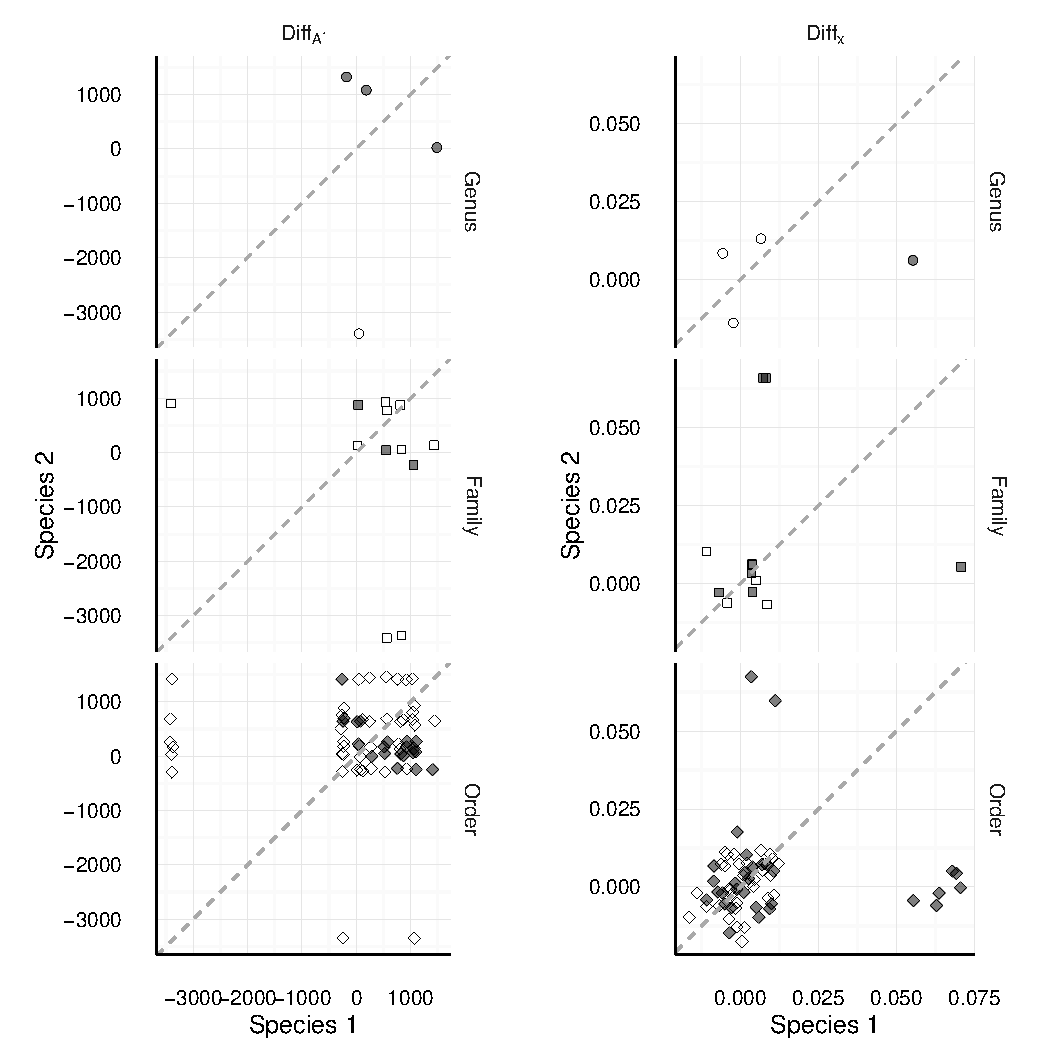
\includegraphics[width=5.5in]{figures/pairwise_astars.pdf}
\caption{Pairwise differences in two measures of size response. Each point represents a
pair of species, divided into species pairs within the same genus (top)
the same family (middle) and order (bottom). The left panel shows
differences in \(A^{*}\) values (units are ml) while the right panel
shows differences in \(x\) (slopes of logistic regression). Species
pairs which are different from a null model are shaded.}
\label{fig:pairwise}
\end{figure}

\begin{figure}[htbp]
\centering
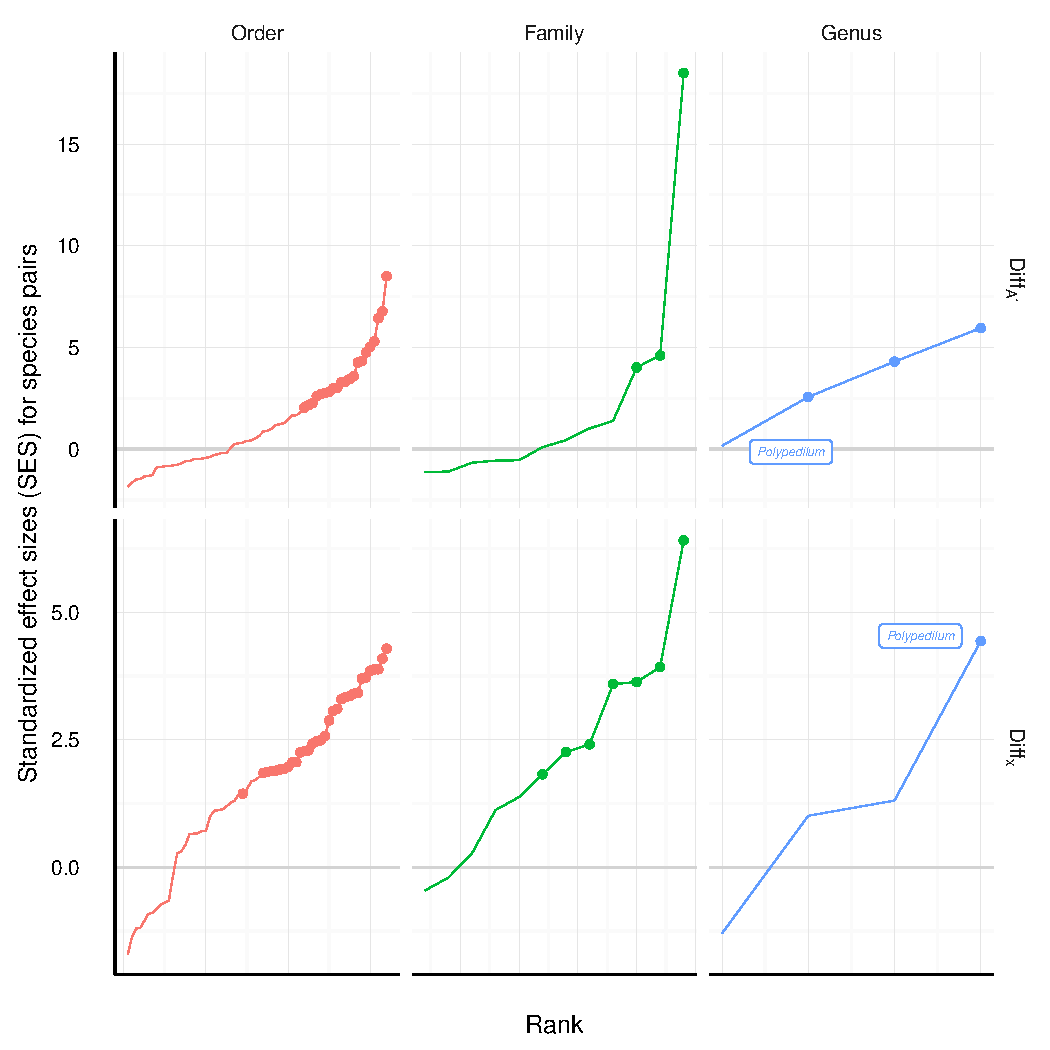
\includegraphics[width=5.5in]{figures/ses_rank.pdf}
\caption{Standardized effect sizes (SES) of pairwise differences
between species for two different measures of patch size response.
These two measures are critical patch size (\(A^{*}\)) and strength of
patch size dependency (\(x\)). Pairwise differences are shown within
each of three taxonomic levels. Significant standardized effect sizes
(randomization p-value \textless{} 0.05) are indicated with points.}
\end{figure}


\end{document}

%%% Local Variables:
%%% TeX-master: t
%%% TeX-PDF-mode: t
%%% End:
